\documentclass[sigconf]{acmart}
% =============================================================================
% Template setup — participants normally do not edit this file.
% Author content belongs in main.tex; citations belong in main.bib.
% \documentclass lives in main.tex so Overleaf does not treat this file as root.
% =============================================================================

% --- Competition / non-ACM-submission friendly rights metadata -------------
\setcopyright{none}
\settopmatter{printacmref=false}
\acmConference[Kaggle Competition]{Filament Segmentation Challenge}{2026}{\href{https://www.kaggle.com/competitions/filament-segmentation-2026}{kaggle.com/competitions/filament-segmentation-2026}}
\acmBooktitle{Competition Report}
\acmDOI{}
\acmISBN{}

% --- Author guidance text --------------------------------------------------
% \guide{...} is gray italic while \guideStyletrue; omitted from the PDF if false.
% Flip the switch in main.tex after % =============================================================================
% Template setup — participants normally do not edit this file.
% Author content belongs in main.tex; citations belong in main.bib.
% \documentclass lives in main.tex so Overleaf does not treat this file as root.
% =============================================================================

% --- Competition / non-ACM-submission friendly rights metadata -------------
\setcopyright{none}
\settopmatter{printacmref=false}
\acmConference[Kaggle Competition]{Filament Segmentation Challenge}{2026}{\href{https://www.kaggle.com/competitions/filament-segmentation-2026}{kaggle.com/competitions/filament-segmentation-2026}}
\acmBooktitle{Competition Report}
\acmDOI{}
\acmISBN{}

% --- Author guidance text --------------------------------------------------
% \guide{...} is gray italic while \guideStyletrue; omitted from the PDF if false.
% Flip the switch in main.tex after % =============================================================================
% Template setup — participants normally do not edit this file.
% Author content belongs in main.tex; citations belong in main.bib.
% \documentclass lives in main.tex so Overleaf does not treat this file as root.
% =============================================================================

% --- Competition / non-ACM-submission friendly rights metadata -------------
\setcopyright{none}
\settopmatter{printacmref=false}
\acmConference[Kaggle Competition]{Filament Segmentation Challenge}{2026}{\href{https://www.kaggle.com/competitions/filament-segmentation-2026}{kaggle.com/competitions/filament-segmentation-2026}}
\acmBooktitle{Competition Report}
\acmDOI{}
\acmISBN{}

% --- Author guidance text --------------------------------------------------
% \guide{...} is gray italic while \guideStyletrue; omitted from the PDF if false.
% Flip the switch in main.tex after \input{preamble}.
%
% Do not use \guide{...} for \email{...}.
\usepackage{xcolor}
\newif\ifguideStyle
\guideStyletrue
\newcommand{\guide}[1]{%
  \ifguideStyle
    {\color{gray!65}\itshape #1}%
  \fi
}

% --- Math ------------------------------------------------------------------
% Do NOT load amssymb (or amsfonts): acmart already loads newtxmath, which
% defines the same symbols (e.g. \Bbbk) and causes a conflict on Overleaf.
% amsmath is already provided by acmart; mathtools extends it.
\usepackage{mathtools}

% --- Figures ---------------------------------------------------------------
% graphicx is already loaded by acmart
\usepackage{subcaption}

% --- Tables ----------------------------------------------------------------
% booktabs is already loaded by acmart
\usepackage{tabularx}
\usepackage{multirow}

% --- Bibliography style is set in main.tex (ACM-Reference-Format) ----------
.
%
% Do not use \guide{...} for \email{...}.
\usepackage{xcolor}
\newif\ifguideStyle
\guideStyletrue
\newcommand{\guide}[1]{%
  \ifguideStyle
    {\color{gray!65}\itshape #1}%
  \fi
}

% --- Math ------------------------------------------------------------------
% Do NOT load amssymb (or amsfonts): acmart already loads newtxmath, which
% defines the same symbols (e.g. \Bbbk) and causes a conflict on Overleaf.
% amsmath is already provided by acmart; mathtools extends it.
\usepackage{mathtools}

% --- Figures ---------------------------------------------------------------
% graphicx is already loaded by acmart
\usepackage{subcaption}

% --- Tables ----------------------------------------------------------------
% booktabs is already loaded by acmart
\usepackage{tabularx}
\usepackage{multirow}

% --- Bibliography style is set in main.tex (ACM-Reference-Format) ----------
.
%
% Do not use \guide{...} for \email{...}.
\usepackage{xcolor}
\newif\ifguideStyle
\guideStyletrue
\newcommand{\guide}[1]{%
  \ifguideStyle
    {\color{gray!65}\itshape #1}%
  \fi
}

% --- Math ------------------------------------------------------------------
% Do NOT load amssymb (or amsfonts): acmart already loads newtxmath, which
% defines the same symbols (e.g. \Bbbk) and causes a conflict on Overleaf.
% amsmath is already provided by acmart; mathtools extends it.
\usepackage{mathtools}

% --- Figures ---------------------------------------------------------------
% graphicx is already loaded by acmart
\usepackage{subcaption}

% --- Tables ----------------------------------------------------------------
% booktabs is already loaded by acmart
\usepackage{tabularx}
\usepackage{multirow}

% --- Bibliography style is set in main.tex (ACM-Reference-Format) ----------


% Guide styling disabled for final submission
\guideStylefalse

\begin{document}

\title[Native-Resolution Solar Filament Panoptic Cascade]{Astrophysics-Calibrated Native-Resolution Panoptic Cascade with Two-Tier Dinkelbach Antichain Selection}
\subtitle{A Solution to the Solar Filament Segmentation Challenge 2026} % DO NOT CHANGE

\author{Timur Shakurov}
\affiliation{%
\city{Almaty}
\country{Kazakhstan}
}
\email{shakurtimur@gmail.com}

\begin{abstract}
    This report describes our solution to the Solar Filament Segmentation Challenge~2026, a Kaggle competition on automatic segmentation of solar filaments in GONG H-$\alpha$ observations. We present a four-stage, strictly pixel-disjoint panoptic cascade operating at native $1{:}1$ solar-disk resolution ($1856\times 1856$ centered window retaining $100\%$ of ground-truth pixels) with zero external metadata at inference. First, per-image astrophysical calibration removes limb darkening and cloud vignetting via a 720-ray IRLS limb fit, 256-bin equal-$u=(r/R)^2$ radial normalization, and two-pass feature-masked flat-fielding. Second, a 5-family calibrated dual-head dense ensemble (25 models, 200 $D_4$ test views/pixel) with exact Law-of-Total-Variance inter-fold disagreement restoration is paired with a 5-fold \texttt{YOLO11l-seg} detector. Third, a 16-level strictly subset-monotone Component Tree extracts 77 photometric, morphological, uncertainty, and detector-agreement descriptors scored by 120 nested Hurdle GBDTs (\texttt{LightGBM}, \texttt{CatBoost}, \texttt{XGBoost}) and decoded via a novel hierarchy-consistent Two-Tier Antichain Dynamic Program. Finally, a 40-model multi-generation PCA-oriented $384\times 128$ conditional refiner (160 views/filament) with \texttt{join3} MST gap bridging and survivor-only \texttt{argmax} serialization yields strictly non-overlapping masks (\texttt{many\_to\_one = 0}). Our system reaches $0.4683$ five-fold OOF Panoptic Quality ($95\%$ CI $[0.4591, 0.4763]$), $0.4676$ strict nested LOFO PQ, $0.7017$ semantic micro-Dice (vs.\ $0.3399$ human pairwise PQ), $0.41$ Public LB, and $0.39$ Private LB (Top-12, Team \texttt{MXlop}). Code and weights are publicly available at \url{https://github.com/little-ruffy/solar-filament-segmentation-2026} and \url{https://huggingface.co/CToraq/solar-filament-segmentation-2026}.
\end{abstract}

\maketitle
\emergencystretch=1.5em

% ==================================== %
%              INTRODUCTION            %
% ==================================== %
\section{Introduction}
    This report goes over the details of our submitted solution to the Solar Filament Segmentation Challenge~2026 \cite{filament-segmentation-2026}. The challenge, launched on July~10,~2026, is organized by the Earth-Space AI Research (ESAIR) Lab\footnote{\href{https://www.esairlab.com/home}{www.esairlab.com/}}. This challenge utilizes the MAGFiLO dataset for evaluation of the segmentation algorithms \cite{ahmadzadeh2024dataset}.

    Exploratory analysis of the 707 training observations (1,154 multi-annotator records; 8,199 polygons across six GONG stations) exposed four core challenges under Panoptic Quality ($\mathrm{PQ}@0.5$) \cite{kirillov2019panoptic}: (1) median filament width is only $11.1\text{ px}$ at $2048^2$, so downsampling blurs thin ribbons and pushes boundary IoU below $0.5$; (2) strong radial Center-to-Limb Variation (CLV) and cloud vignetting vary widely across observatories; (3) multi-annotator subjectivity creates a human pairwise ceiling of $\mathrm{PQ}=0.3399$, requiring calibrated soft consensus modeling; and (4) fixed thresholding either fragments curved filaments or merges adjacent structures. Our cascade resolves all four bottlenecks while strictly enforcing zero pixel overlap ($\mathrm{many\text{-}to\text{-}one}=0$) and leak-free nested validation.

% ==================================== %
%              METHODOLOGY             %
% ==================================== %
\section{Methodology}\label{sec:methodology}

\begin{figure*}[t]
    \centering
    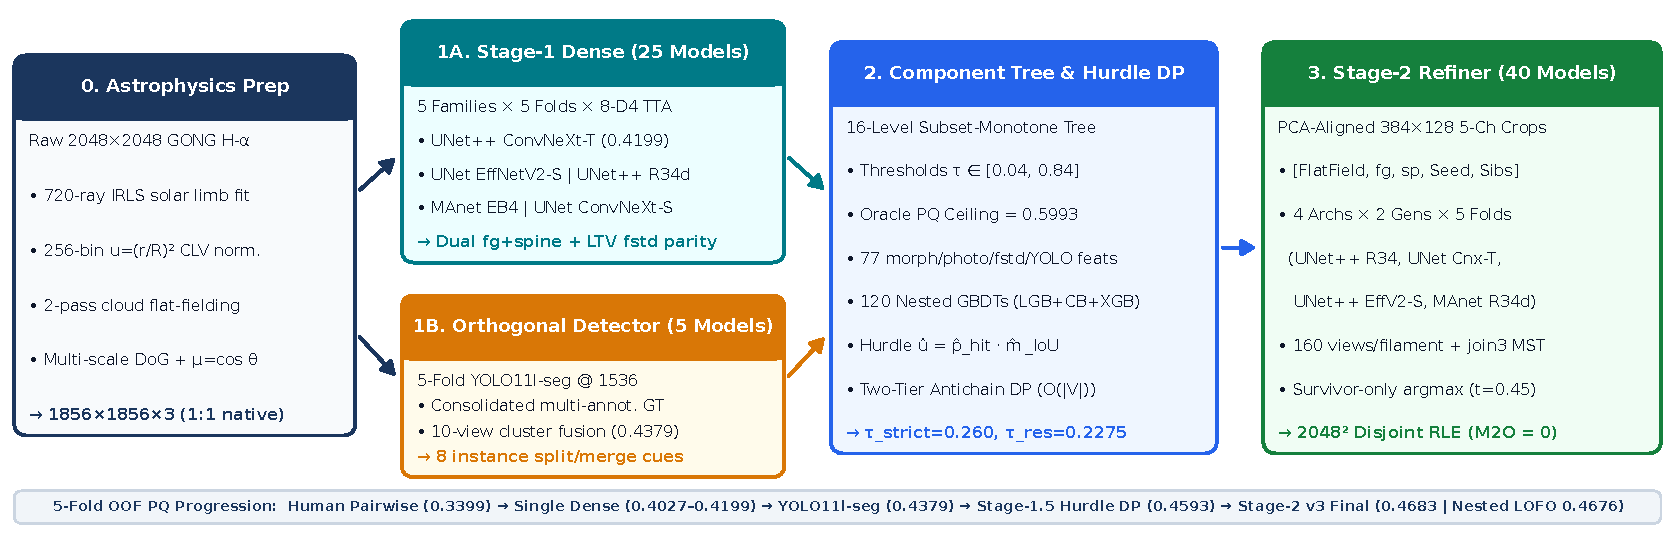
\includegraphics[width=0.96\textwidth]{figures/fig1_pipeline.pdf}
    \vspace{-4pt}
    \caption{End-to-end zero-retraining architecture of our panoptic solar filament segmentation cascade (190 trained models total: 25 Stage-1 dense models, 5 \texttt{YOLO11l-seg} detectors, 120 nested Hurdle GBDTs, and 40 Stage-2 PCA-oriented conditional refiners).}
    \label{fig:pipeline}
    \vspace{-4pt}
\end{figure*}

Figure~\ref{fig:pipeline} illustrates our complete end-to-end data and modeling pipeline. Every preprocessing and inference operator runs strictly per single raw $2048\times 2048$ GONG H-$\alpha$ JPEG without external metadata or cross-frame coupling.

\subsection{Sampling Strategy \& Leak-Free Cross-Validation}
The training set comprises $N=707$ unique physical timestamps annotated by $R_i \in \{1, 2, 3\}$ independent experts ($58.1\%$ $R{=}1$, $20.5\%$ $R{=}2$, $21.4\%$ $R{=}3$; $1,154$ records total), while the test set contains $180$ observations from the same 2011--2022 solar-cycle era and six GONG stations (\texttt{Bh, Ch, Lh, Mh, Th, Uh}). To mirror the host observation-level split and block multi-annotator leakage, we build a 5-fold observation-grouped split stratified jointly on station, $R_i$, filament-count tertile, and solar era ($141\text{--}142$ disks/fold, $0$ shared timestamps across folds). All dense ensemble weights, 120 Hurdle GBDTs (5 outer $\times$ 4 inner early-stopping splits), Dinkelbach thresholds, and Stage-2 slot weights are cross-fitted strictly Leave-One-Fold-Out (LOFO), and every hyperparameter choice is gated by strict Nested LOFO PQ.

\subsection{Stage 0: Astrophysical H-$\alpha$ Calibration}
Across all 8,199 training polygons, the maximum vertex radius from disk center $(1023.5, 1023.5)$ is $903.3\text{ px}$ (median disk radius $R=902.9\text{ px}$). We therefore extract a centered $1856\times 1856$ crop ($[96{:}1952]^2$, divisible by 64), retaining $100.000\%$ of all ground-truth pixels at native $1{:}1$ scale without interpolation blur. For each raw image $I$, our per-image physics module (\texttt{solar\_prep.py}) computes:
\begin{enumerate}
    \item \textbf{720-Ray IRLS Solar Limb Fit:} Casts 720 radial rays ($0.5^\circ$ spacing) over $r\in[760,960]$, detects steepest negative radial gradients, and fits $(c_x, c_y, R)$ via 4-step iteratively reweighted least squares (median RMS $1.01\text{ px}$, robust to clouds where Otsu fails).
    \item \textbf{256-Bin Equal-$u$ CLV Normalization:} Divides intensities by the median radial profile $L(u)$ over 256 bins uniform in $u=(r/R)^2$ ($2\times$ denser sampling near the steep solar limb) to form $I_{\text{clv}} = I / L(u)$.
    \item \textbf{Two-Pass Feature-Masked Cloud Flat-Fielding:} Estimates smooth atmospheric background $B(x)$ via $1/8$-scale Gaussian smoothing ($\sigma=0.10R$), masking dark filaments and bright plages ($|I_{\text{clv}}/B_0 - 1| > 2.5\cdot\text{MAD}$) before Pass~2, yielding calibrated contrast $c(x)=\mathrm{clip}(I_{\text{clv}}/B - 1, -0.45, +0.25)$.
\end{enumerate}
The resulting 3-channel $D_4$-equivariant tensor stacks: (Ch0) flat-field intensity $F(x)=1+c(x)$, (Ch1) isotropic multi-scale Difference-of-Gaussians absorption $(G_{14}-G_{0.8}) + 0.5(G_{4.5}-G_{0.8})$ accentuating $4\text{--}32\text{ px}$ ribbons, and (Ch2) heliocentric foreshortening $\mu(x)=\sqrt{\max(0, 1-u)}$ (zero off-disk).

\subsection{Stage 1: Native Dense Ensemble, LTV Parity \& Detector}
\textbf{Calibrated 5-Family Whole-Disk Dense Ensemble (25 Models).}
Because $100\%$ of MAGFiLO annotations include explicit \texttt{spine} polylines, each Stage-1 network predicts two aligned channels: soft annotator-mean foreground $p(x)=\frac{1}{R_i}\sum_r \mathbf{1}[x\in G_{i,r}]$ and dilated centerline spine $s(x)$. On $1856^2$ disks where filaments cover only ${\sim}0.20\%$ of pixels, standard unweighted $\mathrm{BCE}+\mathrm{SoftDice}$ lets Dice dominate logit gradients by ${\sim}30\times$ and collapses soft probabilities to $\{0,1\}$. We balance logit gradient magnitudes via
\begin{equation}
\begin{aligned}
\mathcal{L} &= \bigl(20\,\mathrm{BCE}_{\text{disk}} + 0.40\,\mathrm{SoftDice}_{\text{disk}}\bigr)_{\text{fg}} \\
            &\quad + 0.30\,\bigl(20\,\mathrm{BCE}_{\text{disk}} + 0.40\,\mathrm{SoftDice}_{\text{disk}}\bigr)_{\text{sp}},
\end{aligned}
\end{equation}
evaluated strictly inside the solar disk with $\mathrm{pos\_weight}=1.0$. Five diverse families are trained with a progressive whole-disk curriculum ($12\text{ ep}@1344 \to 8\text{ ep}@1856$, AdamW differential LRs, cosine decay, EMA, $D_4$ augmentations): UNet++ with ConvNeXt-Tiny \cite{zhou2018unetpp,liu2022convnet} (LOFO weight $0.380$), UNet with EfficientNetV2-S \cite{tan2021efficientnetv2} ($0.228$), UNet++ with ResNet34d ($0.179$), UNet with ConvNeXt-Small ($0.164$), and MAnet with EfficientNet-B4 \cite{fan2020manet} ($0.049$). Both OOF and Test maps use identical 8-view $D_4$ TTA (200 views/pixel on test).

\begin{figure*}[t]
    \centering
    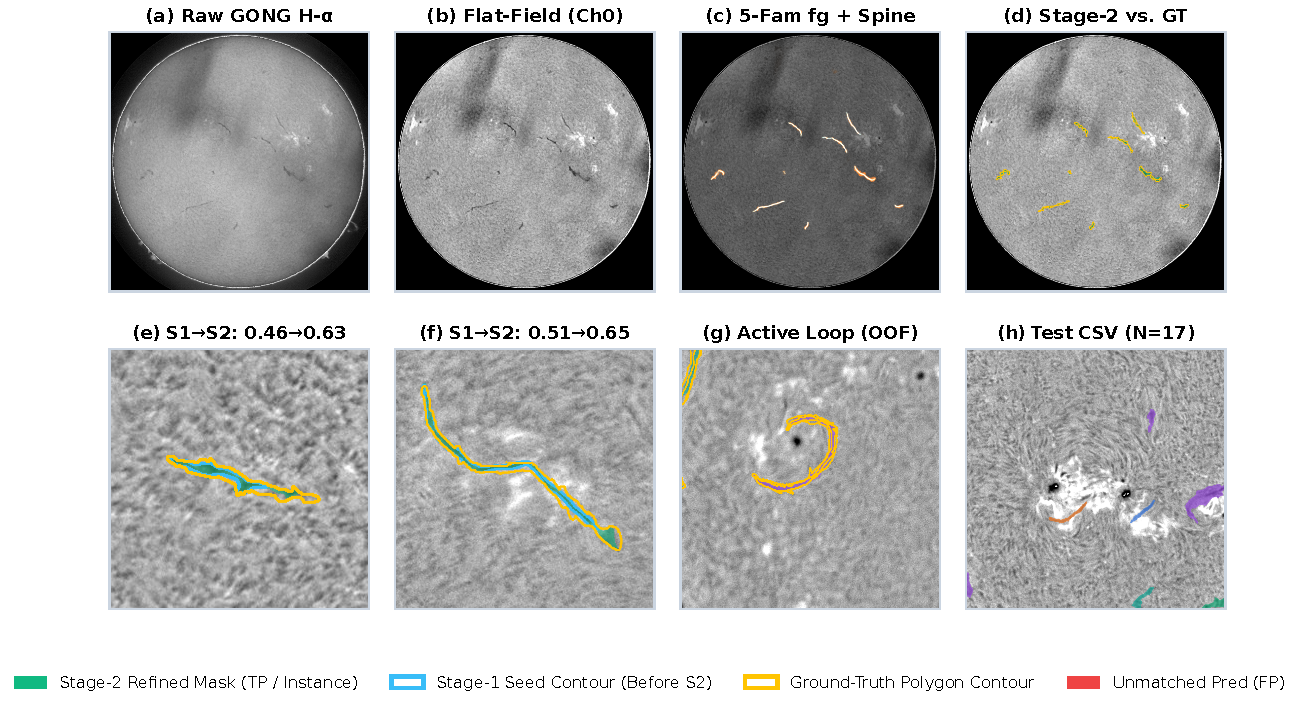
\includegraphics[width=0.71\textwidth]{figures/fig2_qualitative_examples.pdf}
    \vspace{-5pt}
    \caption{Qualitative Stage-2 OOF segmentation examples across three diverse GONG observations: (top) high-activity multi-filament disk, (middle) multi-annotator ($R{=}2$) curved ribbons, and (bottom) challenging low-contrast/ambiguous frame ($R{=}3$). Green masks mark matched true positives ($\mathrm{IoU}>0.5$), red marks unmatched predictions, and gold contours trace union ground-truth polygons.}
    \label{fig:qualitative}
    \vspace{-6pt}
\end{figure*}

\textbf{Exact Law-of-Total-Variance (\texttt{fstd}) Test Parity.}
Because OOF maps come from $1$ fold model per family whereas Test maps average $K{=}5$ folds, cross-family variance $\mathrm{Var}_m(\bar{p}_m)$ shrinks by $-18.8\%$ on Test, causing downstream GBDTs to over-trust borderline test detections. Storing each family's per-pixel inter-fold standard deviation $\mathrm{fstd}_m$ on Test and applying the exact Law-of-Total-Variance correction,
\begin{equation}
\mathrm{Var}_{\text{corr}}(x) = \mathrm{Var}_m(\bar{p}_m(x)) + \frac{M-1}{M}\,\frac{1}{M}\sum_{m=1}^{M}\mathrm{fstd}_m(x)^2,
\end{equation}
restores $\frac{1}{K} + \frac{K-1}{K} = 1.0$ of single-fold variance identically, reducing OOF-to-Test discrepancy in \texttt{fam\_std\_corr} from $-18.80\%$ to $-0.11\%$.

\textbf{Orthogonal Top-Down Detector (5 Models).}
To supply complementary instance separation cues without duplicating multi-annotator polygons, we consolidate overlapping training masks ($\mathrm{IoU}\ge 0.35$) per timestamp and train 5-fold \texttt{YOLO11l-seg} \cite{jocher2024yolo11} at $1536\text{ px}$ ($\mathrm{mask\_ratio}{=}2$, 10 consolidated test views). Rather than injecting coarser YOLO masks directly into the pixel tree (verified $-0.0003$ Nested PQ), we feed 8 detector-node IoU, confidence, containment, and overlap-count features into the Hurdle GBDT.

\subsection{Stage 1.5: Subset-Monotone Tree, Hurdle GBDTs \& Two-Tier Antichain DP}
Under pixel-disjoint predictions ($\mathrm{many\text{-}to\text{-}one}=0$), every predicted instance adds exactly $+\frac{1}{2}$ to the PQ denominator $\mathrm{TP}+\frac{1}{2}\mathrm{FP}+\frac{1}{2}\mathrm{FN} = \frac{1}{2}|P|+\frac{1}{2}|G|$. By Dinkelbach's fractional programming theorem \cite{dinkelbach1967nonlinear}, global PQ maximization decouples per observation into maximizing $\sum_{c\in A_i} (u_i(c) - \tau^*)$ over disjoint subsets $A_i$, with $\tau^* \approx \mathrm{PQ}^*/2$ and expected matched utility
\begin{equation}
u_i(c) = \frac{1}{R_i}\sum_{r=1}^{R_i}\max_{g\in G_{i,r}} \mathrm{IoU}(c,g)\,\mathbf{1}\bigl[\mathrm{IoU}(c,g)>0.5\bigr].
\end{equation}

We construct a 16-level Component Tree over blended foreground thresholds $\{0.04, 0.07, \dots, 0.84\}$ bottom-up via $M_k = \mathrm{Fill}(\mathrm{Close}(p\ge t_k)) \cup M_{k+1}$, mathematically guaranteeing strict parent-child inclusion ($c_{\text{child}}\subseteq c_{\text{parent}}$) and $100\%$ sibling disjointness (Oracle Tree PQ $= 0.5993$ across 111,487 train nodes). For every node we extract 77 features across six groups: probability/spine calibration (22), H-$\alpha$ photometry and disk geometry (14), ribbon morphology/PCA width (12), $D_4$ and LTV-\texttt{fstd} uncertainty (13), tree persistence/topology (8), and YOLO11l-seg agreement (8).

Because $u_i(c)$ has a point mass at $0$, we factor $\hat{u}(c)=\hat{p}_{\text{hit}}(c)\cdot\hat{m}_{\text{IoU}}(c)$ using three GBDT families---\texttt{LightGBM} \cite{ke2017lightgbm}, \texttt{CatBoost} \cite{prokhorenkova2018catboost}, and \texttt{XGBoost} \cite{chen2016xgboost}---cross-fitted over 5 outer $\times$ 4 inner splits (120 models) weighted by $R_i$ and blended on active candidates ($\mathrm{lgb}=0.298, \mathrm{cb}=0.222, \mathrm{xgb}=0.480$). To hand candidates to Stage~2 without shattering intact filaments (an over-splitting failure seen when lowering a single-pass DP threshold), we introduce \textbf{Two-Tier Antichain Handoff}: (1) solve exact $O(|V|)$ bottom-up tree DP at minimax-regret $\tau_{\text{strict}}=0.2600$, locking confident instances; (2) block all ancestors and descendants of locked nodes; and (3) run a second antichain DP at $\tau_{\text{rescue}}=0.2275$ strictly on disjoint remaining subtrees, preserving $100\%$ of Stage-1 DP PQ ($0.4593$) with zero over-splitting.

\subsection{Stage 2: 40-Model PCA-Oriented Refiner \& Disjoint RLE}
To refine thin $4\text{--}11\text{ px}$ boundaries conditioned on each selected instance, we align every candidate along its PCA major axis with $1.30\times$ padding into a canonical $384\times 128$ 5-channel crop containing FlatField, blended \texttt{fg}, blended \texttt{spine}, target seed mask, and competing sibling seed masks. Channel~5 explicitly marks adjacent confident filaments so the refiner never bleeds into neighboring instances. Four diverse encoder-decoder architectures---\texttt{UNet++ ResNet34}, \texttt{UNet ConvNeXt-Tiny}, \texttt{UNet++ EfficientNetV2-S}, and \texttt{MAnet ResNet34d}---are trained across two multi-generation ensembles (5 folds $\times$ 8 slots $= 40$ models, $\mathrm{BCE}+0.65\,\mathrm{SoftDice}$ on conditional matched-annotator masks $q_c(x)$, 4-flip TTA $= 160$ views/filament) and blended via LOFO simplex weights. Inverse-warped probabilities are thresholded at $t_{\text{pix}}=0.45$ ($\alpha_{\text{s2}}=1.0$), sub-pieces separated by $<4\text{ px}$ over dense support ($\mathrm{fg}\ge 0.12$) are bridged via \texttt{join3} MST corridors, and final masks are painted onto a single $2048^2$ \texttt{owner\_map} strictly over surviving candidates ($\hat{u}\ge 0.2600$, protecting confident cores from speculative rescue seeds) resolved by pixelwise \texttt{argmax} probability before canonical Fortran-order COCO RLE encoding. Figure~\ref{fig:qualitative} displays qualitative examples from raw H-$\alpha$ through final pixel-disjoint Stage-2 overlays.

% ==================================== %
%              EVALUATION              %
% ==================================== %
\section{Evaluation}\label{sec:evaluation}

\begin{figure*}[t]
    \centering
    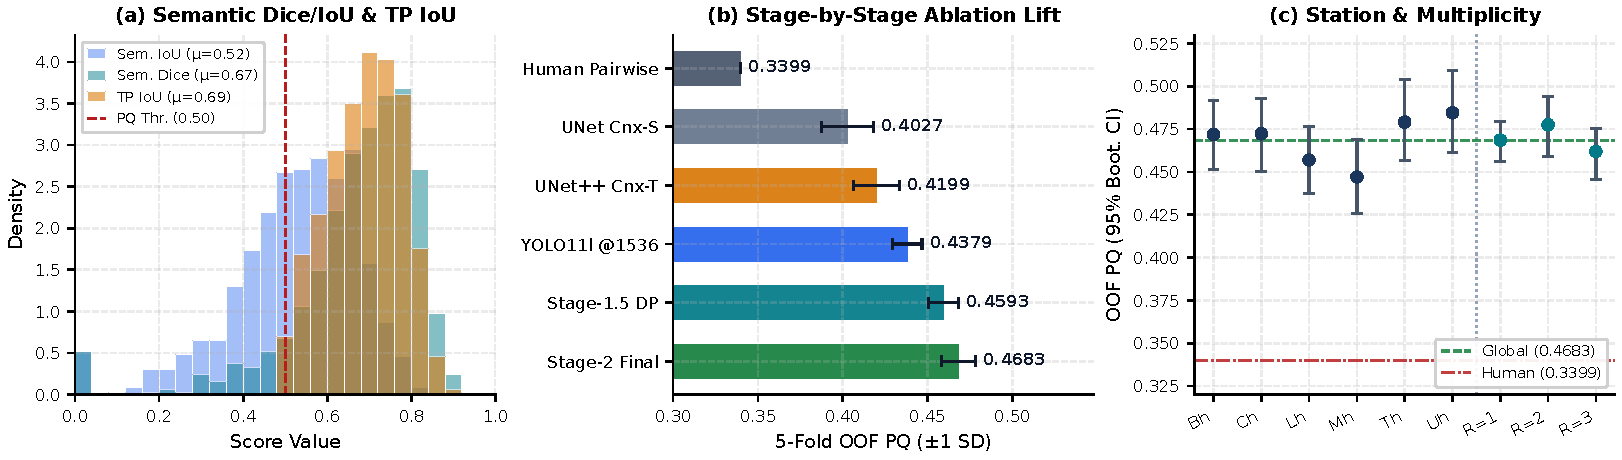
\includegraphics[width=0.90\textwidth]{figures/fig3_evaluation_distributions.pdf}
    \vspace{-5pt}
    \caption{Quantitative evaluation with uncertainty measures on 5-fold OOF predictions (707 disks, 1,154 records): (a) per-record semantic Dice and matched TP IoU distributions relative to the $\mathrm{IoU}>0.5$ threshold; (b) stage-by-stage PQ lift with $\pm 1\text{ SD}$ across folds; (c) cross-observatory (6 GONG stations) and annotator-multiplicity ($R\in\{1,2,3\}$) OOF PQ with 95\% bootstrap CIs.}
    \label{fig:eval}
    \vspace{-6pt}
\end{figure*}

\subsection{Validation Protocol \& Quantitative Results}
We evaluate strictly out-of-fold across all $707$ training disks ($1,154$ annotator records) using a C-accelerated exact replica of the host metric (verified $<10^{-6}$ parity with the competition evaluator). Alongside micro-pooled $\mathrm{PQ}$, $\mathrm{SQ}$, and $\mathrm{RQ}$, we report global and per-record semantic binary Dice, matched instance IoU and Dice distributions, exact one-to-many and many-to-one relation counts, 5-fold standard deviations, and 1,000-resample observation-level bootstrap $95\%$ confidence intervals.

\begin{table}[t]
\centering
\caption{Stage-by-stage 5-fold OOF ablation and Kaggle leaderboard progression. All models use observation-grouped CV and yield zero overlapping pixels (\texttt{M2O = 0}).}
\label{tab:ablation}
\scriptsize
\setlength{\tabcolsep}{3.0pt}
\begin{tabular}{@{}lcccccc@{}}
\toprule
\textbf{Pipeline Stage / Model} & \textbf{OOF PQ} & \textbf{5-Fold SD} & \textbf{SQ} & \textbf{RQ} & \textbf{Pub.} & \textbf{Priv.} \\
\midrule
Human Pairwise (1,196 pairs) & 0.3399 & --- & 0.6337 & 0.5364 & --- & --- \\
\midrule
Stage-1 \texttt{UNet ConvNeXt-S} & 0.4027 & 0.0153 & 0.6741 & 0.5974 & --- & --- \\
Stage-1 \texttt{MAnet EffNet-B4} & 0.4040 & 0.0112 & 0.6634 & 0.6090 & --- & --- \\
Stage-1 \texttt{UNet++ ResNet34d} & 0.4119 & 0.0118 & 0.6710 & 0.6139 & --- & --- \\
Stage-1 \texttt{UNet EffNetV2-S} & 0.4132 & 0.0124 & 0.6745 & 0.6126 & --- & --- \\
Stage-1 \texttt{UNet++ ConvNeXt-T} & 0.4199 & 0.0136 & 0.6736 & 0.6233 & --- & --- \\
Stage-1 \texttt{YOLO11l-seg} @1536 & 0.4379 & 0.0088 & 0.6739 & 0.6499 & --- & --- \\
\midrule
Stage-1.5 Tree+Hurdle DP (v3) & 0.4593 & 0.0090 & 0.6839 & 0.6716 & --- & --- \\
Full Cascade v1 (3-Fam+2-S2) & 0.4669 & 0.0098 & 0.6860 & 0.6806 & 0.40 & 0.38 \\
Full Cascade v2 (+LTV+4-S2) & 0.4678 & 0.0097 & 0.6871 & 0.6808 & 0.41 & 0.38 \\
\textbf{Full Cascade v3 (Final)} & \textbf{0.4683} & \textbf{0.0099} & \textbf{0.6883} & \textbf{0.6804} & \textbf{0.41} & \textbf{0.39} \\
\quad \textit{Strict Nested LOFO (v3)} & \textit{0.4676} & \textit{0.0101} & \textit{0.6883} & \textit{0.6794} & --- & --- \\
\bottomrule
\end{tabular}
\end{table}

Table~\ref{tab:ablation} demonstrates monotonic gains at every stage: upgrading from single-family native dense decoding ($0.4027\text{--}0.4199$) to our 5-family Component Tree + 120-GBDT Hurdle Two-Tier DP yields $+0.0394$ OOF PQ ($0.4593$, Nested LOFO $0.4587$), and Stage-2 40-model oriented refinement adds another $+0.0090$ OOF PQ to reach $\mathbf{0.4683}$ (Nested LOFO $\mathbf{0.4676}$, $+0.0014$ over v2), translating directly into our $0.38 \to 0.39$ Private LB jump (Top-12). Across all $180$ test images, our exact submitted file (\texttt{submission.csv}, 1,196 rows, $6.64$ instances/disk, $177$ active and $3$ quiet disks) passes 14-check RLE validation with $0$ overlapping pixels and closely matches OOF density ($6.50$/disk).

\begin{table}[t]
\centering
\caption{Metric distributions, uncertainty bounds, instance relation audit (1,154 records), and area-quartile sensitivity on Stage-2 v3 OOF predictions.}
\label{tab:dist}
\scriptsize
\setlength{\tabcolsep}{3.0pt}
\begin{tabular}{@{}lcc@{}}
\toprule
\textbf{Metric / Audit Dimension} & \textbf{Point / Mean $\pm$ SD} & \textbf{Median [IQR] / 95\% CI} \\
\midrule
Global OOF PQ (707 disks) & $0.4683 \pm 0.0099$ & 95\% CI $[0.4591, 0.4763]$ \\
Semantic Micro-Dice (union) & $0.7017 \pm 0.0167$ & 95\% CI $[0.6937, 0.7112]$ \\
Per-Record Dice ($n{=}1154$) & $0.6721 \pm 0.1557$ & $0.7070\; [0.6181, 0.7764]$ \\
Matched TP IoU ($n{=}5336$) & $0.6883 \pm 0.0868$ & $0.6948\; [0.6243, 0.7561]$ \\
Matched TP Dice ($n{=}5336$) & $0.8122 \pm 0.0621$ & $0.8199\; [0.7687, 0.8611]$ \\
\midrule
Many-to-One (1,154 recs) & \textbf{0 (0.00\%)} & Disjointness invariant \\
One-to-Many (1,154 recs) & \textbf{1 (0.09\%)} & 1 overlapping GT pair \\
\midrule
Area Q1 ($<670\text{ px}^2$) & Recall $50.9\%$ & Matched SQ $= 0.6829$ \\
Area Q2 ($670\text{--}1228\text{ px}^2$) & Recall $68.1\%$ & Matched SQ $= 0.6843$ \\
Area Q3 ($1228\text{--}2438\text{ px}^2$) & Recall $71.8\%$ & Matched SQ $= 0.6870$ \\
Area Q4 ($\ge 2438\text{ px}^2$) & Recall $69.5\%$ & Matched SQ $= 0.6974$ \\
\bottomrule
\end{tabular}
\end{table}

Table~\ref{tab:dist} and Figure~\ref{fig:eval} report full score distributions and subgroup stability. Matched true positives achieve high boundary fidelity (median IoU $0.6948$, median Dice $0.8199$), semantic micro-Dice reaches $0.7017$ (95\% CI $[0.6937, 0.7112]$), and structural consistency is near-perfect: $\mathbf{0}$ many-to-one events across all 1,154 records and only $1$ one-to-many event (from two overlapping GT polygons with mutual $\mathrm{IoU}=0.724$ inside record \texttt{010403-20160810234034Lh}). Cross-observatory generalization stays tightly consistent across all six GONG sites (Figure~\ref{fig:eval}c, \texttt{Mh} $0.4470$ to \texttt{Uh} $0.4845$, all CIs overlapping the global mean) and across all four annotator codes ($0.4637\text{--}0.4805$) and multiplicities $R\in\{1,2,3\}$ ($0.4619\text{--}0.4775$).

\subsection{Strengths, Weaknesses \& Improvement Strategies}
\textbf{Strengths.}
(1) Native $1856^2$ physics-normalized inputs eliminate downsampling loss and station-specific limb/cloud bias; (2) exact LTV \texttt{fstd} restoration aligns OOF and Test uncertainty features within $0.11\%$; (3) Two-Tier Antichain DP unites Dinkelbach optimality with guaranteed disjointness and zero parent over-splitting; and (4) PCA-aligned Stage-2 refinement lifts $\mathrm{SQ}$ to $0.6883$ while respecting sibling boundaries.

\textbf{Weaknesses.}
(1) Small filaments in the lowest area quartile ($<670\text{ px}^2$, Table~\ref{tab:dist}) show lower recall ($50.9\%$) than medium/large filaments ($68.1\text{--}71.8\%$), where faint fragments blend into chromospheric network noise; (2) a systematic ${\sim}0.06\text{--}0.08$ offset separates multi-annotator OOF PQ ($0.4683$) from single-reference Public and Private LB ($0.41$ / $0.39$) due to human omission variance; and (3) full 190-model inference takes ${\sim}70\text{ s}$/image on an RTX~3090.

\textbf{Future Improvements.}
First, a dedicated high-resolution tile branch around low-contrast active regions can specifically recover small Q1 filaments and barbs. Second, modeling explicit per-annotator strictness priors or test-time precision-recall calibration could better bridge single-annotator shift. Third, distilling our Stage-1 (25 models) and Stage-2 (40 models) ensembles into two compact student networks would retain $>98\%$ of ensemble PQ at $10\times$ faster operational cadence for real-time GONG monitoring.

% ==================================== %
%            ACKNOWLEDGMENT            %
% ==================================== %
\section{Acknowledgment}\label{sec:acknowledgment}
    % Do not change
    The organization of the Filament Segmentation Challenge 2026 is partially supported by the U.S. National Science Foundation (NSF) under Grant No. 2209912 and 2433781, directorate for Computer and Information Science and Engineering (CSE), and Office of Advanced Cyberinfrastructure (OAC), and Grant No. 2511630, AST Division Of Astronomical Sciences and MPS Directorate for Mathematical and Physical Sciences.

    The Filament Segmentation Challenge 2026 is sponsored by the U.S. National Science Foundation (NSF) National Solar Observatory (NSO).

    This work utilizes GONG data obtained by the NSO Integrated Synoptic Program, managed by the National Solar Observatory, which is operated by the Association of Universities for Research in Astronomy (AURA), Inc. under a cooperative agreement with the National Science Foundation and with contribution from the National Oceanic and Atmospheric Administration. The GONG network of instruments is hosted by the Big Bear Solar Observatory, High Altitude Observatory, Learmonth Solar Observatory, Udaipur Solar Observatory, Instituto de Astrofísica de Canarias, and Cerro Tololo Interamerican Observatory.

\bibliographystyle{ACM-Reference-Format}
\bibliography{main}

\end{document}
